%% This file was auto-generated by IPython.
%% Conversion from the original notebook file:
%% lk2.ipynb
%%
\documentclass[11pt,english,fleqn]{article}

%% This is the automatic preamble used by IPython.  Note that it does *not*
%% include a documentclass declaration, that is added at runtime to the overall
%% document.

\usepackage{amsmath}
\usepackage{amssymb}
\usepackage{graphicx}
\usepackage{ucs}
\usepackage[utf8x]{inputenc}

% needed for markdown enumerations to work
\usepackage{enumerate}

% Slightly bigger margins than the latex defaults
\usepackage{geometry}
\geometry{verbose,tmargin=3cm,bmargin=3cm,lmargin=2.5cm,rmargin=2.5cm}

% Define a few colors for use in code, links and cell shading
\usepackage{color}
\definecolor{orange}{cmyk}{0,0.4,0.8,0.2}
\definecolor{darkorange}{rgb}{.71,0.21,0.01}
\definecolor{darkgreen}{rgb}{.12,.54,.11}
\definecolor{myteal}{rgb}{.26, .44, .56}
\definecolor{gray}{gray}{0.45}
\definecolor{lightgray}{gray}{.95}
\definecolor{mediumgray}{gray}{.8}
\definecolor{inputbackground}{rgb}{.95, .95, .85}
\definecolor{outputbackground}{rgb}{.95, .95, .95}
\definecolor{traceback}{rgb}{1, .95, .95}

% Framed environments for code cells (inputs, outputs, errors, ...).  The
% various uses of \unskip (or not) at the end were fine-tuned by hand, so don't
% randomly change them unless you're sure of the effect it will have.
\usepackage{framed}

% remove extraneous vertical space in boxes
\setlength\fboxsep{0pt}

% codecell is the whole input+output set of blocks that a Code cell can
% generate.

% TODO: unfortunately, it seems that using a framed codecell environment breaks
% the ability of the frames inside of it to be broken across pages.  This
% causes at least the problem of having lots of empty space at the bottom of
% pages as new frames are moved to the next page, and if a single frame is too
% long to fit on a page, will completely stop latex from compiling the
% document.  So unless we figure out a solution to this, we'll have to instead
% leave the codecell env. as empty.  I'm keeping the original codecell
% definition here (a thin vertical bar) for reference, in case we find a
% solution to the page break issue.

%% \newenvironment{codecell}{%
%%     \def\FrameCommand{\color{mediumgray} \vrule width 1pt \hspace{5pt}}%
%%    \MakeFramed{\vspace{-0.5em}}}
%%  {\unskip\endMakeFramed}

% For now, make this a no-op...
\newenvironment{codecell}{}

 \newenvironment{codeinput}{%
   \def\FrameCommand{\colorbox{inputbackground}}%
   \MakeFramed{\advance\hsize-\width \FrameRestore}}
 {\unskip\endMakeFramed}

\newenvironment{codeoutput}{%
   \def\FrameCommand{\colorbox{outputbackground}}%
   \vspace{-1.4em}
   \MakeFramed{\advance\hsize-\width \FrameRestore}}
 {\unskip\medskip\endMakeFramed}

\newenvironment{traceback}{%
   \def\FrameCommand{\colorbox{traceback}}%
   \MakeFramed{\advance\hsize-\width \FrameRestore}}
 {\endMakeFramed}

% Use and configure listings package for nicely formatted code
\usepackage{listingsutf8}
\lstset{
  language=python,
  inputencoding=utf8x,
  extendedchars=\true,
  aboveskip=\smallskipamount,
  belowskip=\smallskipamount,
  xleftmargin=2mm,
  breaklines=true,
  basicstyle=\small \ttfamily,
  showstringspaces=false,
  keywordstyle=\color{blue}\bfseries,
  commentstyle=\color{myteal},
  stringstyle=\color{darkgreen},
  identifierstyle=\color{darkorange},
  columns=fullflexible,  % tighter character kerning, like verb
}

% The hyperref package gives us a pdf with properly built
% internal navigation ('pdf bookmarks' for the table of contents,
% internal cross-reference links, web links for URLs, etc.)
\usepackage{hyperref}
\hypersetup{
  breaklinks=true,  % so long urls are correctly broken across lines
  colorlinks=true,
  urlcolor=blue,
  linkcolor=darkorange,
  citecolor=darkgreen,
  }

% hardcode size of all verbatim environments to be a bit smaller
\makeatletter 
\g@addto@macro\@verbatim\small\topsep=0.5em\partopsep=0pt
\makeatother 

% Prevent overflowing lines due to urls and other hard-to-break entities.
\sloppy

\setlength{\mathindent}{0pt}
\setlength{\parindent}{0pt}
\setlength{\parskip}{8pt}
\begin{document}

Piksel Takibi, Optik Akis, Lucas Kanade Algoritmasi

Hareket halindeki bir kameranin aldigi goruntulerdeki herhangi bir
pikseli nasil takip ederiz?

Matematiksel olarak temsil etmek gerekirse, zamana gore degisen 2
boyutlu goruntuyu bir fonksiyon olarak dusunelim, ki bu fonksiyonun
degerleri ayriksal olarak, imajin ta kendisi. Bir $I(x(t),y(t),t)$
fonksiyonu piksel degerlerini veriyor. Bu fonksiyonda $x,y$ ekran
kordinatlarina tekabul ediyor, $t$ ise zaman, $1,2,..$ gibi degerleri
indeks degerleri var, mesela $I(100,200,1)$, bize 1. video karesindeki
$x=100,y=200$ kordinatlarindaki piksel degerini verecek.

$x,y$ degiskenleri parametrize edildi, bir noktayi takip etmek istiyoruz
cunku, ve $t$'ye gore bu takip edilen noktanin $x,y$ kordinatlari belli
bir gidisat yonunde degisiyor.

Su faraziyeyi yaparak takip problemimizi kolaylastirabiliriz. Diyelim ki
takip edilen bir nokta, goruldugu her karede ayni piksel rengindedir. Bu
cok siradisi bir faraziye degil, resim karelerinden bir araba geciyor
mesela, ve bu arabanin uzerindeki piksellerin renkleri, en azindan iki
kare arasinda degismiyor. Isik seviyesi, golgede olma, vs.~gibi
durumlarda biraz degisebilir, fakat basitlestirme amaciyla bu faraziye
gecerlidir.

\begin{codecell}
\begin{codeinput}
\begin{lstlisting}
im=imread("disp2.png"); imshow(im)
\end{lstlisting}
\end{codeinput}
\begin{codeoutput}
\begin{verbatim}
<matplotlib.image.AxesImage at 0xa46cf8c>
\end{verbatim}
\begin{center}
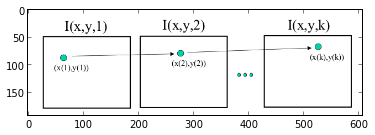
\includegraphics[width=0.7\textwidth]{lk2_files/lk2_fig_00.png}
\par
\end{center}
\end{codeoutput}
\end{codecell}
Bir diger faraziye, kameralar hareket ettiklerinde alinan iki goruntu
arasindaki tum piksellerin yer degisimi genellikle ayni yonde olmasidir.
Bu degisim yonunu $<u,v>$ vektoru olarak gorebiliriz, ve bu degiskenler
iki goruntu arasindaki degisimde tum pikseller icin ayni olacaktir. Bu
da normal, kamerayi alip mesela saga dogru hareket ettiriyoruz, ve
goruntudeki tum pikseller sola dogru gidiyorlar.

\begin{codecell}
\begin{codeinput}
\begin{lstlisting}
im=imread("disp.png"); imshow(im)

\end{lstlisting}
\end{codeinput}
\begin{codeoutput}
\begin{verbatim}
<matplotlib.image.AxesImage at 0xa5c5f2c>
\end{verbatim}
\begin{center}
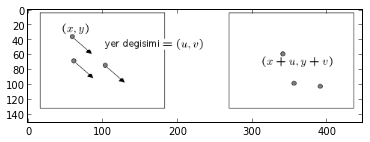
\includegraphics[width=0.7\textwidth]{lk2_files/lk2_fig_01.png}
\par
\end{center}
\end{codeoutput}
\end{codecell}
Tum bunlari modelimizde nasil kullaniriz?

Takip edilen nokta her karede ayni renkte ise, su ifade dogru demektir
\[ I(x(t),y(t),t) = \textrm{ sabit } \]
Eger bu fonksiyonun zamana gore turevini alirsak
\[ \frac{d \ I(x(t),y(t),t)}{dt} = 0\]
sonucu gelir. Esitligin sagi sifir, cunku bir sabitin turevini aldik.
Sol tarafa Zincirleme Kanununu uygularsak,
\[ \frac{\partial I}{\partial x}\frac{dx}{dt} +
\frac{\partial I}{\partial y}\frac{dy}{dt} +
\frac{\partial I}{\partial t} = 0
\]
Bu formulde $dx/dt$ ve $dy/dt$, hareket halindeki (zaman gecerken)
noktanin sonsuz kucuklukteki yer degimi. Ayriksal baglamda arka arkaya
iki kare icindeki yer degisimi. O zaman,
\[ \frac{dx}{dt}, \frac{dy}{dt} = u, v \]
Alttakiler ise mesafesel (spatial) gradyanlardir, bunlarin nasil
hesaplanacagini cok iyi biliyoruz!
\[ 
\frac{\partial I}{\partial x}, \frac{\partial I}{\partial y}
 \]
Alttaki ise resim karelerinin zamana gore turevidir.
\[ 
\frac{\partial I}{\partial t}
 \]
Daha derli toplu olarak gostermek gerekirse ana formul nihai olarak
soyle
\[ I_x u + I_y v + I_t = 0 \]
ya da
\[ 
\nabla I \cdot <u, v> = -I_t
 \]
Simdi $u,v$'nin hesaplanmasina gelelim. Ustteki formulu bir veri noktasi
icin yazmak yeterli degil. Ama bu formulu hem takip ettigimiz, hem de
onun etrafindaki pikseller icin yazarsak (onlarin yer degisimi de ayni
degil mi?), ve bu sistemi cozersek, sonuca varabiliriz.

Iki tane bilinmeyenimiz var, ama boylece pek cok formul elde ediyoruz.
Veriler gurultulu oldugu icin, aslinda bilinmeyenden ``daha fazla''
formul elde etmek iyi, bu tur denklem sistemlerina ``cok esitlige sahip
(overdetermined)'' denir, ve boyle tur sistemler En Az Kareler (Least
Squares) ile cozulur. Tum bunlari biraraya koyunca su ortaya cikar.
\[ 
\left[\begin{array}{cc}
I_x(p_1) & I_y(p_1) \\
I_x(p_2) & I_y(p_1) \\
\vdots & \vdots \\
I_x(p_k) & I_y(p_k) 
\end{array}\right]
\left[\begin{array}{r}
u \\
v
\end{array}\right] = 
-
\left[\begin{array}{c}
I_t(p_1) \\
I_t(p_2) \\
\vdots \\
I_t(p_k) 
\end{array}\right]
 \]
Gradyanlarin belli noktalarda hesaplandigini unutmayalim, o sebeple
$p_1, p_2$ gibi piksel noktalarini bu fonksiyonlara geciyoruz.

Bu sistemi
\[ A \ d = b \]
olarak gosterebiliriz, ki $d = <u,v>$. Sol tarafi $A^T$ ile carpalim
\[ A^TA \ d = A^Tb \]
Eger $A^TA$'nin matris tersini iki tarafla carparsak, $d$ yanliz kalir,
ve sonuc elde edilir.

Bu denklemi Python Numpy'da pinv kullanarak cozeriz.

Test icin uc tane resim kullandik, bu resimlerden flow1-bw-0.png
baslangic resmi, bu resmin ortasindaki objeleri GIMP kullanarak elle
kopyaladik, bir ust sag capraza dogru, bir alt sol capraza dogru, ve iki
yeni resim elde ettik (upright.png, dleft.png). Takip edilen nokta gri
dortgenin alt sol kosesinde. Lucas Kanade algoritmasi bu noktayi takip
ederek, yesil ile isaretledi.

\begin{codecell}
\begin{codeinput}
\begin{lstlisting}
def gauss_kern():
    h1 = 15
    h2 = 15
    x, y = np.mgrid[0:h2, 0:h1]
    x = x-h2/2
    y = y-h1/2
    sigma = 1.5
    g = np.exp( -( x**2 + y**2 ) / (2*sigma**2) );
    return g / g.sum()

def deriv(im1, im2):
    g = gauss_kern()
    Img_smooth = si.convolve(im1,g,mode='same')
    fx,fy=np.gradient(Img_smooth)    
    ft = si.convolve2d(im1, 0.25 * np.ones((2,2))) + \
        si.convolve2d(im2, -0.25 * np.ones((2,2)))
                    
    fx = fx[0:fx.shape[0]-1, 0:fx.shape[1]-1]    
    fy = fy[0:fy.shape[0]-1, 0:fy.shape[1]-1];
    ft = ft[0:ft.shape[0]-1, 0:ft.shape[1]-1];
    return fx, fy, ft

im1 = np.asarray(Image.open('flow1-bw-0.png'))
im2 = np.asarray(Image.open("upright.png"))
fx, fy, ft = deriv(im1, im2)
fx[:5]
\end{lstlisting}
\end{codeinput}
\begin{codeoutput}
\begin{verbatim}
array([[ 34.37477011,  45.94010835,  51.877951  , ...,  53.83264716,
         51.877951  ,  45.94010835],
       [ 26.01168277,  34.76327322,  39.25648957, ...,  40.73562489,
         39.25648957,  34.76327322],
       [ 11.72919465,  15.67546405,  17.70154632, ...,  18.36851839,
         17.70154632,  15.67546405],
       [  3.51803959,   4.70167857,   5.30937909, ...,   5.50942984,
          5.30937909,   4.70167857],
       [  0.6961225 ,   0.93033183,   1.05057892, ...,   1.09016341,
          1.05057892,   0.93033183]])
\end{verbatim}
\end{codeoutput}
\end{codecell}
\begin{codecell}
\begin{codeinput}
\begin{lstlisting}
import numpy as np
import scipy.signal as si
from PIL import Image
import numpy.linalg as lin

def lk(im1, im2, i, j, window_size) :
    fx, fy, ft = deriv(im1, im2)
    halfWindow = np.floor(window_size/2)
    curFx = fx[i-halfWindow-1:i+halfWindow, 
               j-halfWindow-1:j+halfWindow]
    curFy = fy[i-halfWindow-1:i+halfWindow, 
               j-halfWindow-1:j+halfWindow]
    curFt = ft[i-halfWindow-1:i+halfWindow, 
               j-halfWindow-1:j+halfWindow]
    curFx = curFx.T
    curFy = curFy.T
    curFt = curFt.T

    curFx = curFx.flatten(order='F') 
    curFy = curFy.flatten(order='F') 
    curFt = -curFt.flatten(order='F') 
    
    A = np.vstack((curFx, curFy)).T
    U = np.dot(np.dot(lin.pinv(np.dot(A.T,A)),A.T),curFt)
    return U[0], U[1]

def test(image1,image2):        
    x=165
    y=95
    win=50
    im1 = np.asarray(Image.open(image1))
    im2 = np.asarray(Image.open(image2))
    u, v = lk(im1, im2, x, y, win)
    plt.imshow(im1, cmap='gray')
    plt.hold(True)
    plt.plot(x,y,'+r');
    plt.plot(x+u*3,y+v*3,'og')

test("flow1-bw-0.png","dleft.png")

\end{lstlisting}
\end{codeinput}
\begin{codeoutput}
\begin{center}
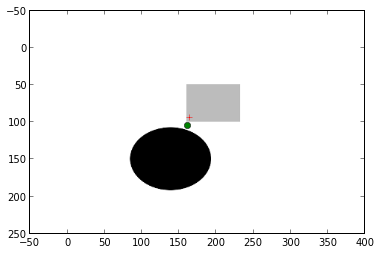
\includegraphics[width=0.7\textwidth]{lk2_files/lk2_fig_02.png}
\par
\end{center}
\end{codeoutput}
\end{codecell}
\begin{codecell}
\begin{codeinput}
\begin{lstlisting}
test("flow1-bw-0.png","upright.png")

\end{lstlisting}
\end{codeinput}
\begin{codeoutput}
\begin{center}
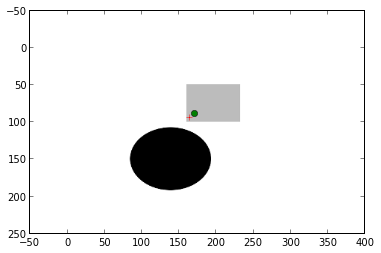
\includegraphics[width=0.7\textwidth]{lk2_files/lk2_fig_03.png}
\par
\end{center}
\end{codeoutput}
\end{codecell}
Not

Bu matematiksel modele alternatif bir bakis soyle olabilir. Iki imaj
karesi icinde birincisine $I(x,y)$ ikincisine $H(x,y)$ diyelim, burada
$t$ uzerinden parametrizasyon olmasin; $x,y$ pikselinin $H$ icinde $u,v$
kadar yer degisiminden sonra, bu noktalarin $I$'de geldigi yerdeki
grilik degerinin ayni oldugunu (yine) farzediyoruz. Sonra
$I(x+u,y+v)$'nin birinci dereceden Taylor Acilimini yapiyoruz,
\[ I(x+u,y+v) = I(x,y) + \frac{\partial I}{\partial x}u + 
\frac{\partial I}{\partial y}v + ...
\]
ya da
\[ I(x+u,y+v) \approx I(x,y) + \frac{\partial I}{\partial x}u + 
\frac{\partial I}{\partial y}v 
\]
Grilik ayniligini ise soyle belirtebiliriz
\[  I(x+u,y+v) - H(x,y) = 0\]
Taylor acilini ustteki formulde $I$ yerine gecirelim
\[ I(x,y) + 
\frac{\partial I}{\partial x}u + 
\frac{\partial I}{\partial y}v - H(x,y) = 0
\]
$H$'in yerini degistirelim
\[ I(x,y)  - H(x,y) + I_xu + I_yv = 0\]
Su ifade $I(x,y) - H(x,y)$ nedir? Bunlar iki imajin, sonrasi ve oncesi
arasindaki fark degil midir? O zaman bu hesabi imajin zamana gore
alinmis turevi olarak gorebiliriz, yani $I_t = I(x,y) - H(x,y)$. Yerine
koyalim
\[ I_t + I_xu + I_yv = 0\]\[ I_xu + I_yv = -I_t \]
Boylece ayni denkleme erismis olduk. Bu aslinda normal, birinci
dereceden Taylor acilimi ile tam diferansiyel denklemi (ve Zincirleme
Kanununu) birbiriyle cok yakindan alakasi var.

Kaynaklar

R. Collins Ders Notlari,
www.cse.psu.edu/\ensuremath{\sim}rcollins/CSE486

Khurram Hassan-Shafique, CAP 5415 Lecture Notes, Spring 2003

http://dl.dropbox.com/u/1570604/skfiles/campy/chessb-left.avi

\end{document}
